\documentclass[twoside]{article}
\usepackage{package}
\usepackage[T1]{fontenc}
\usepackage{subfiles}
% Silenciar la advertencia de versalita + negrita inexistente
\WarningFilter{latex}{Some font shapes were not available}
\WarningFilter{latex}{Font shape `T1/lmr/bx/sc'}

% Silenciar la advertencia de caracteres perdidos en el nullfont (para 01_introduccion.tex)
\WarningFilter{latex}{Missing character: There is no}
%Nuevos comandos
\renewcommand{\thefootnote}{\arabic{footnote}}
\raggedbottom



\begin{document}
\begin{center}
    \thispagestyle{empty}
    \large{\textsc{Matrices en MATLAB y Respuesta Transitoria}}\\[0.5cm] 
    \large{Fabrizio Benavidez\footnote[1]{\texttt{fabrizio.benavidez@mi.unc.edu.ar}}}\\[0.5cm]

    \large{\footnotemark[1]\textit{Facultad de Ciencias Exactas, Físicas y Naturales, Ingeniería Aeronáutica}}
    \\[0.5cm]

    \begin{minipage}{0.7\textwidth}
    \hrule
    \vspace{0.2cm}
        \normalsize{\textsc{Resumen}. El siguiente trabajo práctico representa la manipulación y creación de matrices y vectores usados en MATLAB. Además, se utiliza los ciclos para la generación de gráficas en un \texttt{subplot}, así como la función \texttt{zpk} para generar funciones de transferencias en base a sus ganancias, ceros y polos. Este último fue necesario para el análisis en la respuesta transitoria para distintas configuraciones de un sistema de segundo orden.}\\[0.2cm]
        \normalsize{\textit{Palabras claves}: ciclos \texttt{for}, \texttt{subplot}, \texttt{zpk}, respuesta transitoria.\ }
    \vspace{0.2cm}
    \hrule
    \end{minipage}
    
    \vfil

    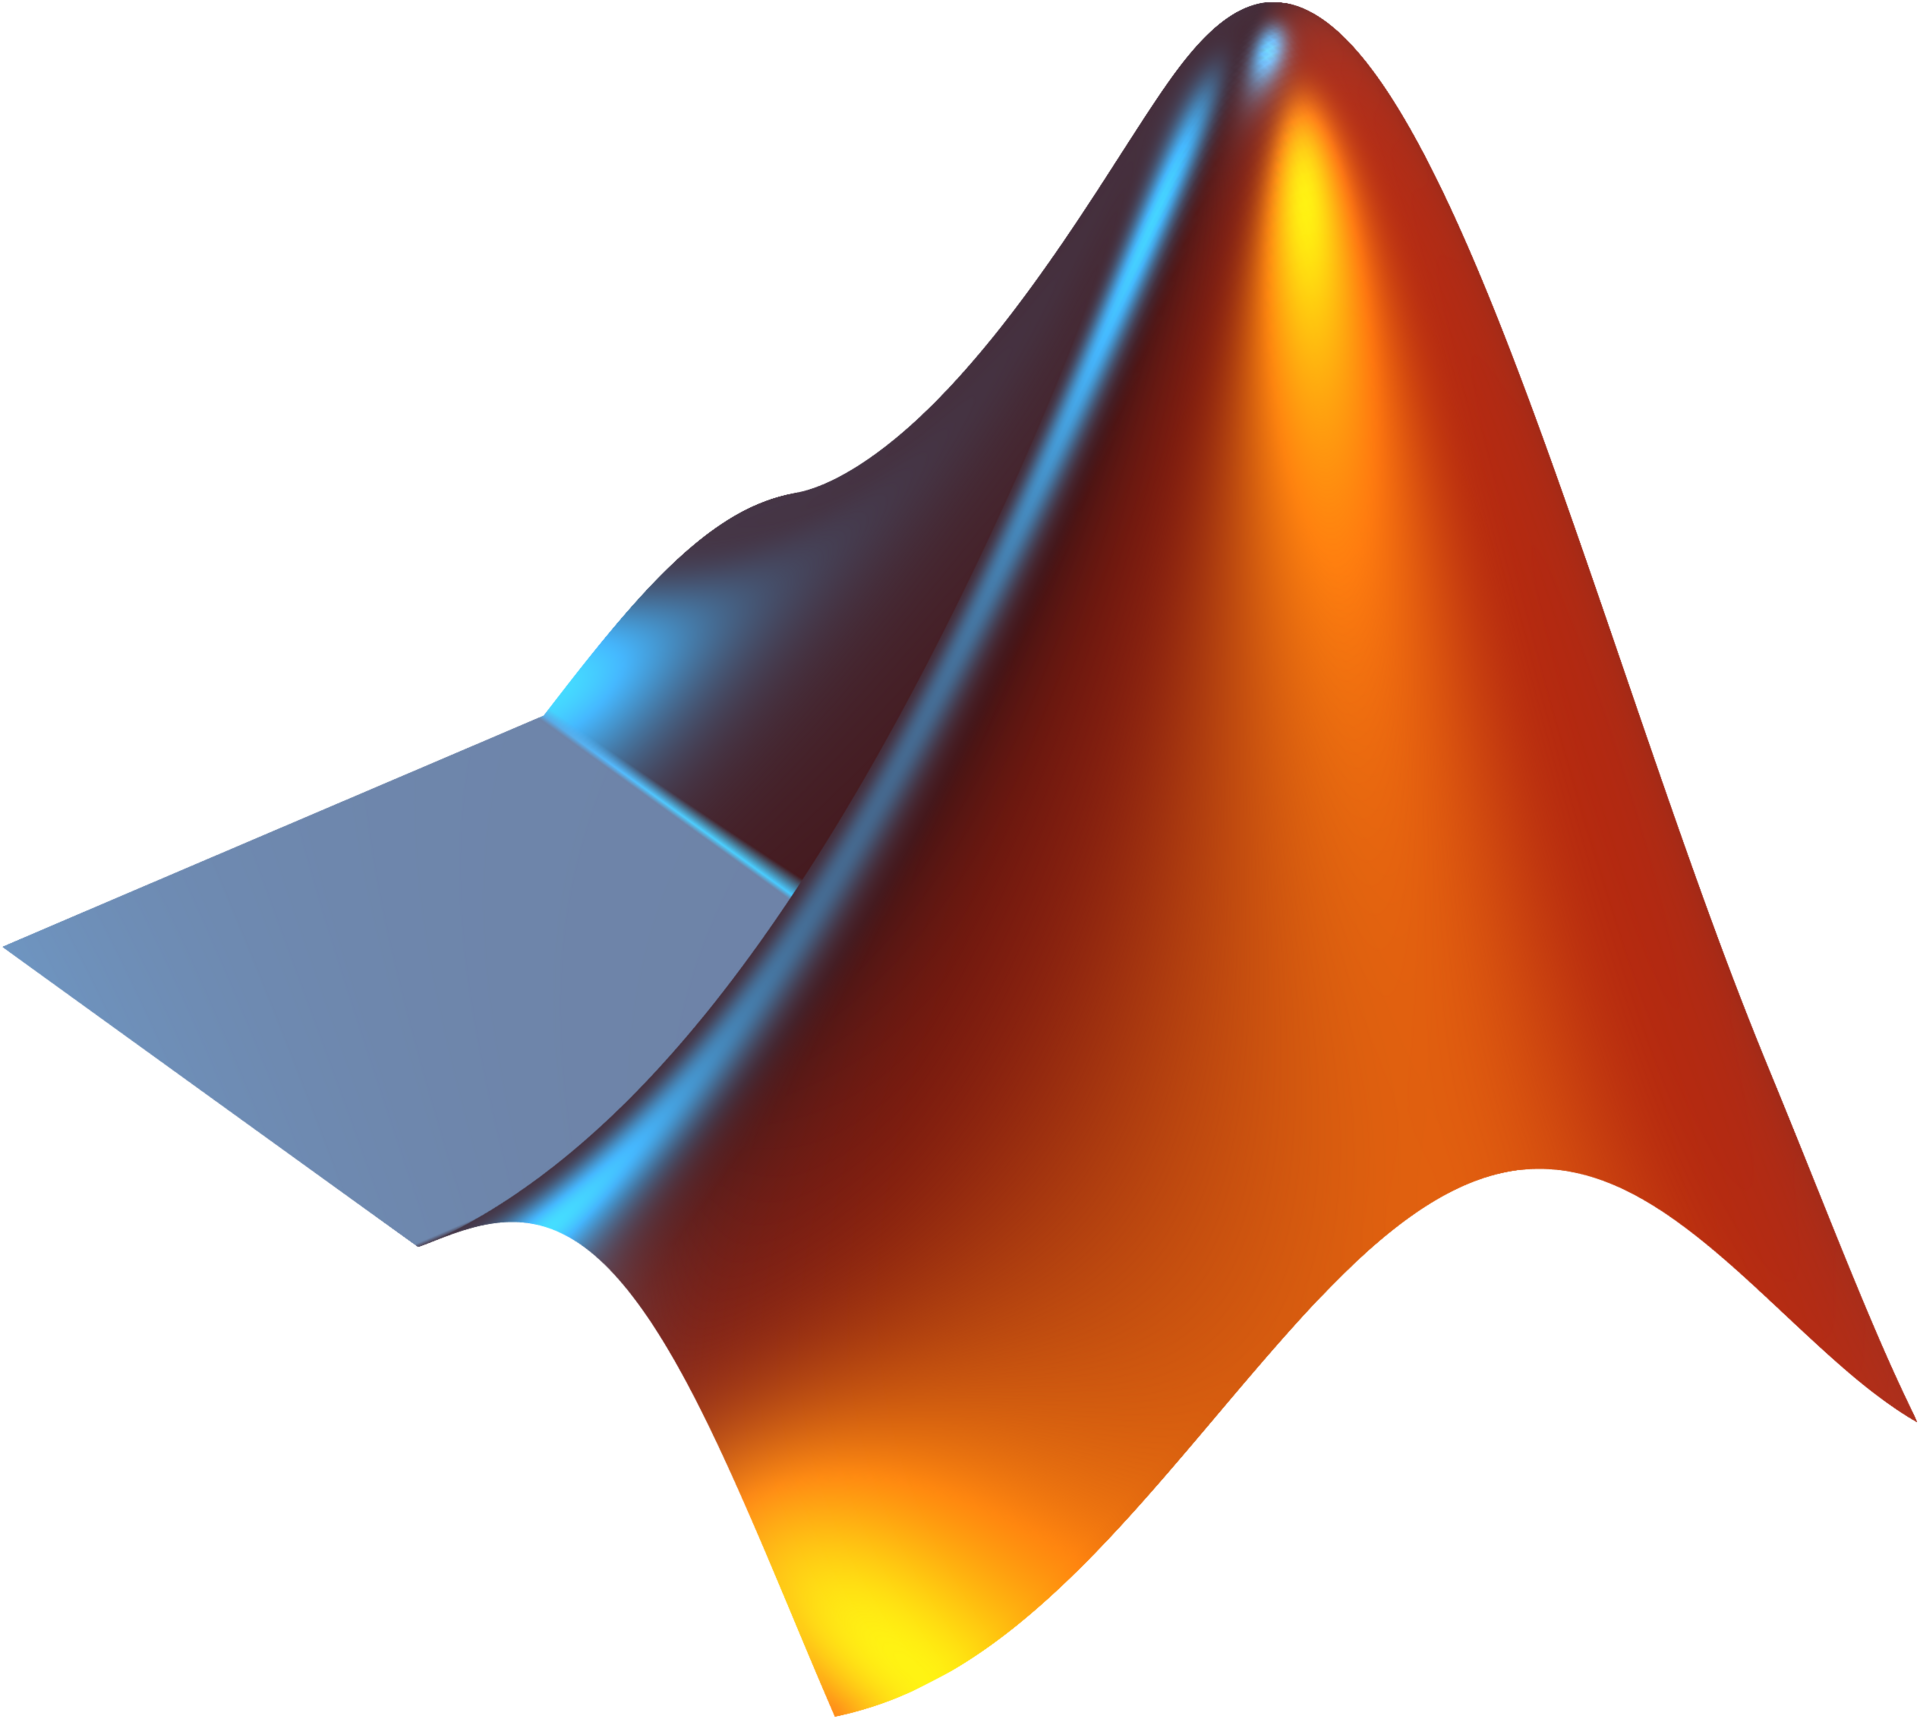
\includegraphics[width = 0.4\textwidth]{imagenes/Matlab_Logo.png}\\[0.5cm]

    \vfil

    \today\\[0.2cm]
    \large{Semana 4}
\end{center}





\newpage

\section*{Guía 07} 
\subfile{secciones/guia07}

\newpage

\section*{Guía 08} 
\subfile{secciones/guia08}














\newpage
\thispagestyle{empty}
\bibliography{biblioteca.bib}
\bibliographystyle{plain}


\end{document}